\documentclass[../main.tex]{subfiles}

\begin{document}


\chapter{概述}
\vspace{-2cm}

简要总结

\section{BasicSR介绍}

正文在这里

\textbf{粗体}

\uline{下划线}
\newline

\textbf{以下摘自:https://zhuanlan.zhihu.com/p/261223409 。 需要修改}

国庆长假期间, 琢磨着想给 BasicSR 代码库写个教程, 于是便开了一个专栏, 方便之后周末抽空慢慢更新.

你看到这里可能会问, BasicSR 是什么, 用来干啥的, 后面会有什么发展. 在这篇概述里面, 就先来聊聊这些问题, 以及这个专栏之后打算写些什么内容.

1. BasicSR介绍
BasicSR 是读博期间写论文、打比赛过程中的codes慢慢沉淀下来的一个代码库. 我之前主要是做超分辨率 (简称超分, Super-Resolution, SR)的, 因此从名字BasicSR就可以猜测出当时起名字的时候, 是全称 Basic Super-Resolution的缩写.

那为什么要加上Basic呢? 最开始想名字的时候, 想的是OpenSR, 用意是开源 Open Source. 这个名字蛮好, 但当时很心虚, 因为自己很清楚, 当时的很多算法, 包括自己参加比赛的、发论文的, 都还是停留在学术研究中, 有很强的前提假设. 远远不能解决实际中复杂多变的问题. 我担心OpenSR这个名字太宏大, 人们把算法拿来一用, 发现这些个算法根本没法用到实际场景中, 那心里便要犯嘀咕了.

当时便想, 退而求其次吧, 就先准备一个基础的库, Basic, 这是最基本的, 要是用在实际环境中, 还得要继续改进, 所以便叫 BasicSR 了.

有 BasicSR, 自然就有与之对应的 AdvancedSR, 这里面的SR算法便要足够advanced, 能够解决真实世界中的复杂问题. 不仅要解决, 还要解决好, 更要有智能. 当时是很期待等自己毕业的时候, 能够有 AdvancedSR 这一个代码库, 然后, 就没有然后了 =-=||

这也算是个初心吧, 留待后面慢慢来做了.

在实际问题中, SR往往是不会单独出现的, 它往往是和去噪, 去模糊, 去压缩等复杂的降质 (降低质量) 的过程一起存在的. 所以我们也不会仅仅单独考虑超分. 之后, BasicSR 和 AdvancedSR 是要将这些都综合考虑进来. 因此: SR不仅仅是Super-Resolution, 我更愿意称他们为SuperRestoration.


目前 AdvancedSR 暂时不考虑了, 先把 BasicSR 拉扯大再说=-= 东西用久了, 还是会有感情的, 有时候想想, 它可能还真像个小孩子似的, 看着一点点发生变化, 有种老父亲的感觉=-= 所以呢, 自己会用着它, 用久了顺手; 也会在周末假期抽空来维护一下.

总之, BasicSR是一个开源的专注图像和视频复原的代码库.

2. BasicSR目标
照着最开始的想法, BasicSR 是为了方便研究者的. 因此之前很多写法, 设计都是以方便做实验来做的, 这个后面也会一直保持. 我平时是使用 BasicSR 来开发新算法、做实验的, 因此会把自己觉得好用的、便捷的设计放进去. 这些改动也都是经过自己试验的, 每个改动都会有个来由, 为解决某个小问题而改动的.

理想情况下, BasicSR 给研究者用, AdvancedSR 会尽可能的方便简单, 给不熟悉算法的人用. 这不, AdvancedSR 还没有出生嘛. 因此呢, 之后也会逐渐把能够应用到实际场景中的算法, 慢慢放在 BasicSR 中, 也会添加方便的测试脚本和Google Colab的脚本.

我现在依旧做着图像和视频的复原工作, 而且会朝着实际应用的方向走. 加上我平时也用BasicSR 来开发, 因此这个代码库的发展路径会不可避免地受到自己研究的关注点的影响. 我会将自己正在使用的, 复现的, 尝试的一些代码逐渐merge到 BasicSR 里面.

总之, BasicSR 一方面以研究者为中心, 不断将自己看到的, 跑过的算法加入其中 (只要自己不断在跟研究的话, 这些算法也大概会是前沿的); 另一方面会提供方便用户使用的脚本和说明文档, 朝着AdvancedSR的目标前进.

3. BasicSR现状
目前BasicSR开源在Github上, 项目地址:

xinntao/BasicSR
​github.com/xinntao/BasicSR

为了方便国内使用 (Github网速实在太慢……), 我在Gitee码云上也放了一份代码. 它是Github版本的镜像版本. Gitee码云地址:

Xintao/BasicSR
​gitee.com/xinntao/BasicSR

平时开发, 上传还是用的Github. 一旦有更新, 会触发Github的Action, 自动push到Gitee.

同时, 我也给主要的文档, 都添加了一份中文的文档说明 (以CN.md 结尾), 对很多人来说, 阅读中文的速度会更快. 我会尽可能保证中文的更新和英文是同步的, 但免不了有时候更新了英文了, 忘记了中文的, 欢迎大家帮助修改.

对于模型和数据, 我上传了Google Drive和百度云, 各有一份.

如果你可以上外网, 那么也提供了wandb训练的曲线和log. wandb是类似在线的tensorboard, 很好用. 一些预训练的模型训练曲线就直接放在上面了, 可以查看:

https://app.wandb.ai/xintao/basicsr
​app.wandb.ai/xintao/basicsr
最近也添加了Google Colab, 但这块还刚添加, 内容比较少. 后面有时间会慢慢添加.

https://github.com/xinntao/BasicSR/tree/master/colab
​github.com/xinntao/BasicSR/tree/master/colab

4. 专栏的计划
国庆期间大概列了一下, 这个专栏大概会有以下四个部分:

BasicSR代码解读
这部分主要讲现在 BasicSR 的代码库的代码组织和设计, 可以看作一个扩充版的README. BasicSR 有自己针对底层复原任务的特殊考量, 也借鉴学习了很多优秀的代码库. 在这里尽可能详细的做一个说明, 同时也让自己再看一遍, 和大家讨论一下, 还可以小小地再重构提升一下.

BasicSR如何使用
如何使用BasicSR, 比如, 如何安装, 如何训练模型, 如何新增数据集, 如何新增网络结构和模型等

BasicSR个人经验
这一块主要想分享自己之前读博期间积累的经验, 比如跑实验、管理实验、写code啥的. 还记得刚读博的时候, 我是一个实验copy一份代码+-+, 实验管理很混乱, 有时候结果不好, 都不知道是实验跑错了, 还是本身方法不work. 切身体会, 好的流程、实验管理是非常重要的.

后来也是在老师师兄指导下, 慢慢改进的. 特别是打比赛的经历, 是很能够锻炼这方面的, 因为不注意的话, 大部分的时间就都耗在无用的地方了. 我的个人经验不一定是好的, 很多也是瞎摸索出来的. 和大家一起讨论, 一起来提高流程、实验管理方面的效率, 能够让出更多的时间在解决核心问题上.

BasicSR番外篇
番外篇, 主要打算是绍一些遇到的好的paper, 或者 BasicSR 实现的方法, 有哪些小坑、做过的小探究.






%\setlength{\columnsep}{0.7cm}
\begin{wrapfigure}{r}{0.4\linewidth}
%\vspace{-0.3cm}
\centering
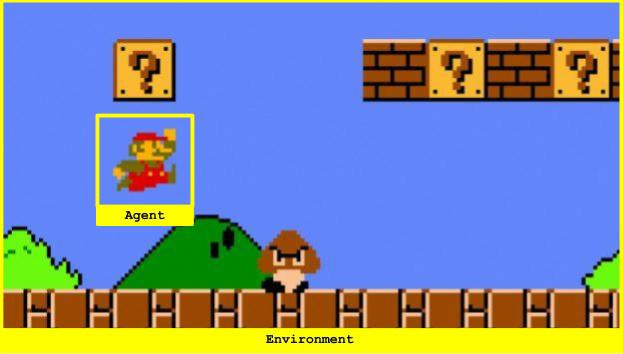
\includegraphics[width=0.4\textwidth]{figures/agentenv.png}
%\caption{Пример среды с двумя действиями.}
%\label{fig:env}
%\vspace{-2.6cm}
\end{wrapfigure}


\begin{hl} 
	\textbf{重要信息可以这么用, 这是总起句}
	
	正常 Latex 使用
	\begin{itemize}
		\item $\St$ --- zzzz.
		\item $\Trans$ --- yyy $\{p(s_{t+1} \HM\mid s_t) \HM\mid t \HM\in \{0, 1, \dots \}, s_t, s_{t+1} \HM\in \St\}$.
	\end{itemize}
\end{hl}

\begin{note} 
	\textbf{Note 信息,这是总起句}
	
	正常 Latex 使用\\
	\href{http://xxx.com}{url}
\end{note}


BasicSR如何使用
如何使用BasicSR, 比如, 如何安装, 如何训练模型, 如何新增数据集, 如何新增网络结构和模型等

BasicSR个人经验
这一块主要想分享自己之前读博期间积累的经验, 比如跑实验、管理实验、写code啥的. 还记得刚读博的时候, 我是一个实验copy一份代码+-+, 实验管理很混乱, 有时候结果不好, 都不知道是实验跑错了, 还是本身方法不work. 切身体会, 好的流程、实验管理是非常重要的.

后来也是在老师师兄指导下, 慢慢改进的. 特别是打比赛的经历, 是很能够锻炼这方面的, 因为不注意的话, 大部分的时间就都耗在无用的地方了. 我的个人经验不一定是好的, 很多也是瞎摸索出来的. 和大家一起讨论, 一起来提高流程、实验管理方面的效率, 能够让出更多的时间在解决核心问题上.

BasicSR番外篇
番外篇, 主要打算是绍一些遇到的好的paper, 或者 BasicSR 实现的方法, 有哪些小坑、做过的小探究.

\begin{exampleBox}[righthand ratio=0.35, sidebyside, sidebyside align=center, lower separated=false]{题目}
	
	示例box,可以放什么东西呢,还没有想好
	
	等后面再看看



\end{exampleBox}


\section{使用场景}

\end{document}